% !TeX root = ../../main.tex
\chapter{Network Editors \who{Neumann, Zilske, Ordóñez}}
\label{ch:networkeditor}
% ##################################################################################################################

\hfill \textbf{Author:} Andreas Neumann, Michael Zilske, Sergio Arturo Ordóñez

\begin{center} 
\includegraphics[width=0.3\textwidth, angle=0]{figures/MATSimBook.png} \end{center}

% ##################################################################################################################
\section{JOSM Network Editor}
This is a plug-in for \citet[][]{JOSM2014}, the Java OpenStreetMap editor, which simplifies the process of creating and editing MATSim networks. The plug-in fully integrates with JOSM and thus benefits from its build-in functionality.

\begin{figure}
\centering
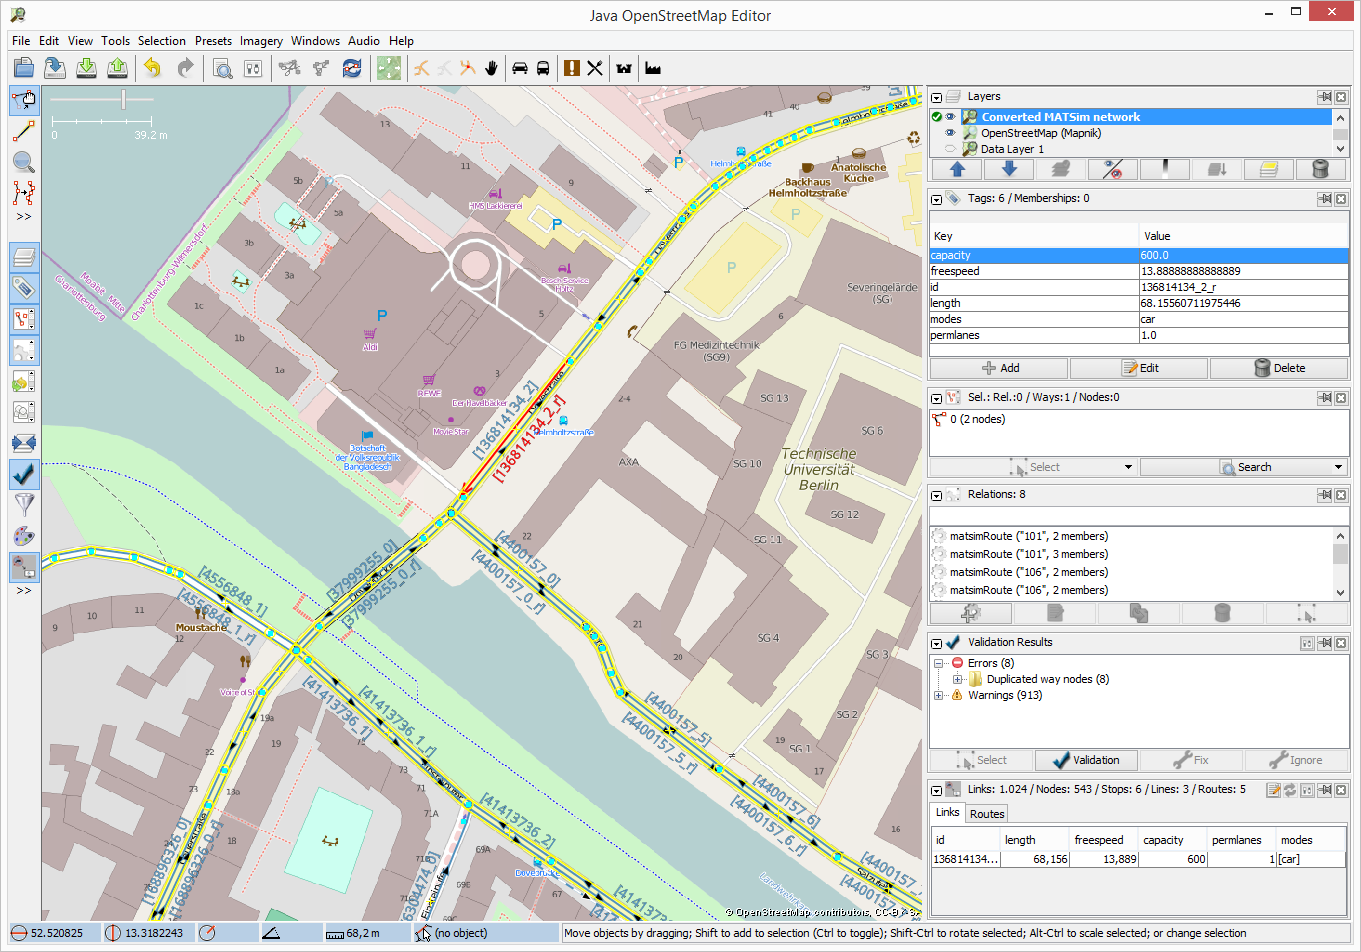
\includegraphics[width=0.9\linewidth]{extending/modules/networkeditor/josm_screenshot.png}
\caption{JOSM with converted MATSim network and OpenStreetMap background imagery. Map data taken from \citet[][]{OpenStreetMap2014}.}
\label{fig:networkeditor_screenshot}
\end{figure}

\subsection{Features}
It lets you preview, edit and save a MATSim network directly from the map. Basic support for converting and editing public transport networks is implemented. The plug-in allows to automatically post-process a network by removing unnecessary intermediate nodes and links.
\begin{description}
\item[Convert] MATSim networks from OpenStreetMapData. Load map data for a selected area directly from the Internet or load it from a local osm file. Specify conversion parameters and save a MATSim network.
\item[Visualize] an existing or newly converted MATSim network along with other data like satellite imagery or other JOSM-supported layers.
\item[Edit] an existing or newly converted MATSim network with the available JOSM tools you know. Use the build-in undo and search functions of JOSM. Changes to the underlying OpenStreetMap data are instantly reflected by the converted MATSim network. Use MATSim-specific presets to minimize errors.
\item[Validate] an existing or newly converted MATSim network with respect to the requirements of the MATSim network file description. Visualize the errors and fix them (automatically). 
\end{description}

\subsection{How to install}
You don't need to download the source to use it. It is in the JOSM plug-in repository. Just start JOSM and look for the MATSim plug-in under Edit$>$Preferences$>$Plugins. Download the list of available plug-ins and search for ``matsim''. Tick the box, press ``ok'' and restart JOSM.

\subsection{How to extend}
The sourcecode is hosted on github (\url{https://github.com/matsim-org/josm-matsim-plugin}). Unlike MATSim, the build is not based on Maven, but on Gradle. The reason is that there are some things to do (like editing the Manifest, downloading JOSM for compilation, and building a flat jar) for which we found a good example in Gradle. Use your favorite IDE to import the Gradle project and/or see the comments in build.gradle for details. You can run JOSM and the plug-in in the debugger.
 
% ##################################################################################################################
\section{Network Editor Singapore}
\citet[][]{Ordonez_Webpage_2011_3}

% ##################################################################################################################